\documentclass[border=1mm]{standalone}
\usepackage[usenames,dvipsnames]{xcolor}
\usepackage{amsmath, amsfonts, amssymb, amsthm}
\usepackage{tikz}
\usetikzlibrary{arrows.meta,shapes,calc,shapes.geometric}
\usetikzlibrary{angles,quotes}
\begin{document}
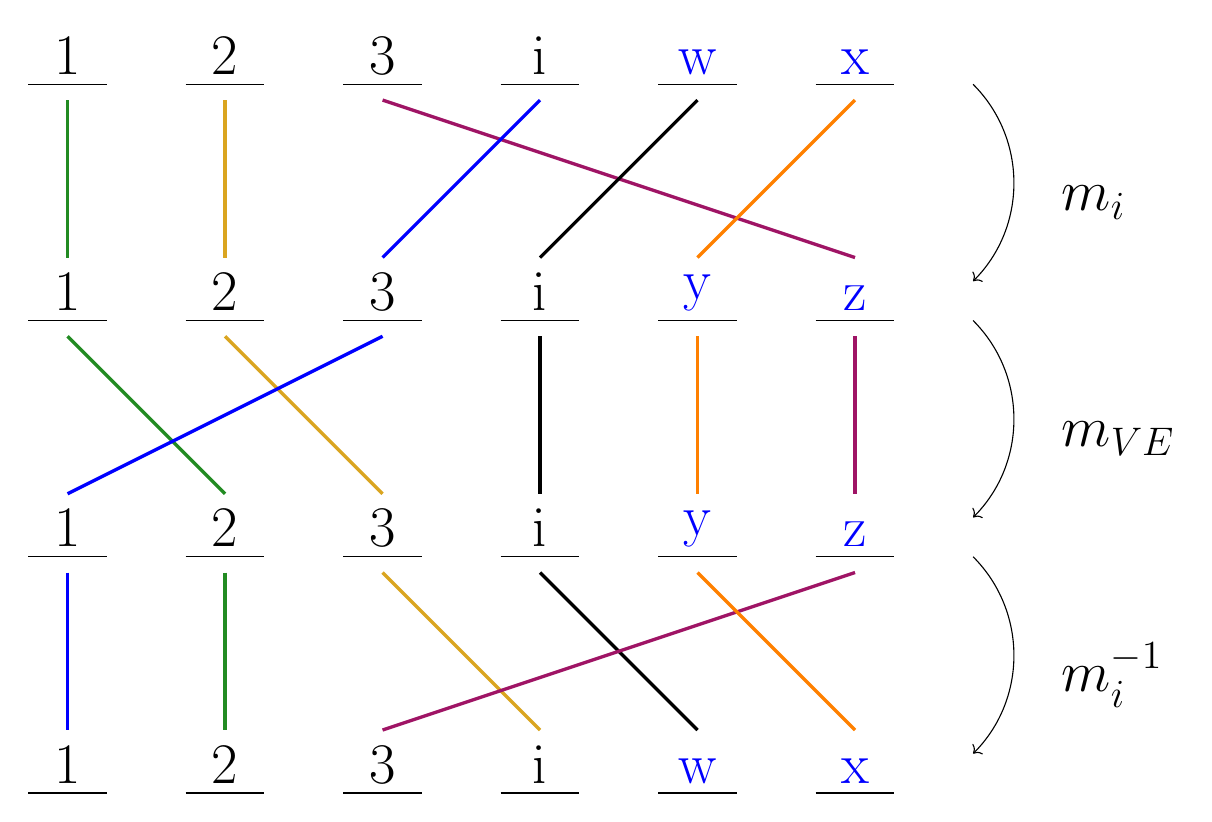
\begin{tikzpicture}
    \draw (0,0) -- node[above]{\huge{1}}(1,0); 
    \draw (2,0) -- node[above]{\huge{2}}(3,0); 
    \draw (4,0) -- node[above]{\huge{3}}(5,0); 
    \draw (6,0) -- node[above]{\huge{i}}(7,0); 
    \draw (8,0) -- node[above]{\textcolor{blue}{\huge{w}}}(9,0); 
    \draw (10,0) -- node[above]{\textcolor{blue}{\huge{x}}}(11,0); 
    \coordinate[label=right: {\huge{$m_i$}}] (m1) at (13, -1.5);
    \draw[->, out=-45, in=45] (12, 0) to (12, -2.5);
    \draw[very thick, ForestGreen] (0.5, -0.2) -- (0.5, -2.2);
    \draw[very thick, Goldenrod] (2.5, -0.2) -- (2.5, -2.2);
    \draw[very thick, RedViolet] (4.5, -0.2) -- (10.5, -2.2);
    \draw[very thick, blue] (6.5, -0.2) -- (4.5, -2.2);
    \draw[very thick, black] (8.5, -0.2) -- (6.5, -2.2);
    \draw[very thick, orange] (10.5, -0.2) -- (8.5, -2.2);
    \begin{scope}[yshift=-3cm]
        \draw (0,0) -- node[above]{\huge{1}}(1,0); 
        \draw (2,0) -- node[above]{\huge{2}}(3,0); 
        \draw (4,0) -- node[above]{\huge{3}}(5,0); 
        \draw (6,0) -- node[above]{\huge{i}}(7,0); 
        \draw (8,0) -- node[above]{\textcolor{blue}{\huge{y}}}(9,0); 
        \draw (10,0) -- node[above]{\textcolor{blue}{\huge{z}}}(11,0); 
        \coordinate[label=right: {\huge{$m_{VE}$}}] (m2) at (13, -1.5);
        \draw[->, out=-45, in=45] (12, 0) to (12, -2.5);
        \draw[very thick, ForestGreen] (0.5, -0.2) -- (2.5, -2.2);
        \draw[very thick, Goldenrod] (2.5, -0.2) -- (4.5, -2.2);
        \draw[very thick, blue] (4.5, -0.2) -- (0.5, -2.2);
        \draw[very thick, black] (6.5, -0.2) -- (6.5, -2.2);
        \draw[very thick, orange] (8.5, -0.2) -- (8.5, -2.2);
        \draw[very thick, RedViolet] (10.5, -0.2) -- (10.5, -2.2);
    \end{scope}
    \begin{scope}[yshift=-6cm]
        \draw (0,0) -- node[above]{\huge{1}}(1,0); 
        \draw (2,0) -- node[above]{\huge{2}}(3,0); 
        \draw (4,0) -- node[above]{\huge{3}}(5,0); 
        \draw (6,0) -- node[above]{\huge{i}}(7,0); 
        \draw (8,0) -- node[above]{\textcolor{blue}{\huge{y}}}(9,0); 
        \draw (10,0) -- node[above]{\textcolor{blue}{\huge{z}}}(11,0); 
        \coordinate[label=right: {\huge{$m_i^{-1}$}}] (m3) at (13, -1.5);
        \draw[->, out=-45, in=45] (12, 0) to (12, -2.5);
        \draw[very thick, blue] (0.5, -0.2) -- (0.5, -2.2);
        \draw[very thick, ForestGreen] (2.5, -0.2) -- (2.5, -2.2);
        \draw[very thick, Goldenrod] (4.5, -0.2) -- (6.5, -2.2);
        \draw[very thick, black] (6.5, -0.2) -- (8.5, -2.2);
        \draw[very thick, RedViolet] (10.5, -0.2) -- (4.5, -2.2);
        \draw[very thick, orange] (8.5, -0.2) -- (10.5, -2.2);
    \end{scope}
    \begin{scope}[yshift=-9cm]
        \draw (0,0) -- node[above]{\huge{1}}(1,0); 
        \draw (2,0) -- node[above]{\huge{2}}(3,0); 
        \draw (4,0) -- node[above]{\huge{3}}(5,0); 
        \draw (6,0) -- node[above]{\huge{i}}(7,0); 
        \draw (8,0) -- node[above]{\textcolor{blue}{\huge{w}}}(9,0); 
        \draw (10,0) -- node[above]{\textcolor{blue}{\huge{x}}}(11,0); 
    \end{scope}
\end{tikzpicture}
\end{document}